\question{}

\begin{ابجد}
\item نمودار حالت به این صورت می‌باشد:
\begin{figure}[H]
    \centering
    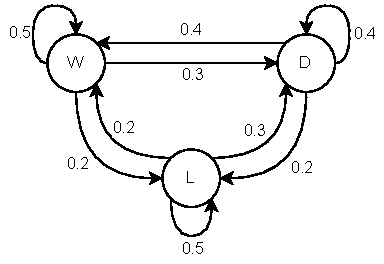
\includegraphics[width=0.6\textwidth]{assets/q3-stateDiagram.pdf}
\end{figure}

\item طبق قاعده‌ی زنجیره‌ای داریم:
\begin{align*}
    P(X_1 = L, X_2 = D, X_3 = W) & = P(X_1 = L) \cdot P(X_2 = D | X_1 = L) \cdot P(X_3 = W | X_2 = D) \\
                                 & = 0.2 \times 0.3 \times 0.4 = 0.024
\end{align*}

\item برای اینکه احتمال برد در مرحله‌ی سوم را محاسبه کنیم، باید احتمال تک‌تک حالت‌های مسابقه‌ی دوم را در احتمال شرطی برد در مسابقه‌ی بعدی به شرط حالت فعلی ضرب کرده و با هم جمع کنیم. برای محاسبه‌ی احتمال تمام حالت‌های مسابقه‌ی دوم نیز باید همین کار را برای هر 3 حالت انجام دهیم. \\
اگر توزیع احتمال حالت‌های یک مسابقه را با ماتریس سطری $\begin{bmatrix} P(W) & P(D) & P(L) \end{bmatrix}$ نمایش دهیم، روشن است که در هر مرحله توزیع احتمال مسابقه‌ی بعدی از ضرب این بردار در ماتریس احتمال انقال حاصل می‌شود.  ماتریس توزیع اولیه به این صورت می‌باشد:
\begin{align*}
    v_1 = \begin{bmatrix} P(X_1 = W) & P(X_1 = D) & P(X_1 = L) \end{bmatrix} = \begin{bmatrix}0.4 & 0.4 & 0.2\end{bmatrix}
\end{align*}
حال توزیع احتمال مسابقه‌های بعدی را محاسبه می‌کنیم:
\begin{align*}
     & v_2 = v_1 \times P = \begin{bmatrix}0.4 & 0.4 & 0.2\end{bmatrix} \times \begin{bmatrix} 0.5 & 0.3 & 0.2 \\ 0.4 & 0.4 & 0.2 \\ 0.2 & 0.3 & 0.5 \end{bmatrix} = \begin{bmatrix}0.4 & 0.34 & 0.26\end{bmatrix}       \\
     & v_3 = v_2 \times P = \begin{bmatrix}0.4 & 0.34 & 0.26\end{bmatrix} \times \begin{bmatrix} 0.5 & 0.3 & 0.2 \\ 0.4 & 0.4 & 0.2 \\ 0.2 & 0.3 & 0.5 \end{bmatrix} = \begin{bmatrix}0.388 & 0.334 & 0.278\end{bmatrix} \\
\end{align*}
بنابراین احتمال برد در مسابقه‌ی سوم برابر است با:
\begin{align*}
    P(X_3 = W) = 0.388
\end{align*}


\end{ابجد}